% -*-coding: utf-8 -*-

Nyní se dostáváme k implementaci námi popsaného formalismu, nazývejme jí dále modelem. Než přikročíme přímo k popisu, musíme dospecifikovat některé požadavky na model a rozebrat ty části algoritmů, které ve formalismu nejsou brány v úvahu, ale pro implementaci jsou důležité. V další kapitole budou následovat příklady konkrétních implementací některých OA.

\section{Specifikace požadavků na model a jeho omezení}

Při implementaci máme některé konkrétní požadavky a některé obecnější myšlenky, které je nutné při programování uvažovat. Chceme:
\begin{itemize}
  \item Pružný objektový model (v průběhu vývoje byl několikrát refaktorován a nelze to vyloučit ani v budoucnu).
  \item Jednoduché přepínání možností kompilace pro GPU a CPU s výhledem na možnost kombinace obou.
  \item Oddělit implementaci od uživatele, ten by měl již pouze \bq skládat kostky\eq  nebo popisovat myšlenky.
  \item Možnost skládat algoritmus z kostek runtime.
  \item Minimalizaci počtu uživatelských parametrů.
  \item Vypořádání se vzhledem k paralelizaci se stavem, kdy výpočet účelové funkce zabere řádově více času, než zbytek algoritmu.
  \item Omezení se na jedince reprezentované vektorem čísel. Tzn. ne stromy, ne struktury proměnlivé velikosti atd.
  \item Účinnou paralelizaci respektující omezení GPU.
  \item Nevynucovat logiku populace-potomstvo tam, kde není nutná.
  \item Jednoduchý výstup poskytující jak výsledky výpočtu, tak případné ladící informace. Předpokládá se zpracování např. v MATLABu.
  \item Omezení se na jednokriteriální optimalizace s perspektivou snadného rozšíření na vícekriteriální.
\end{itemize}

Skládání algoritmu runtime je zásadní požadavek pro další high-level nástavby, avšak k tomuto požadavku jsme se dostali i z druhé strany. Tento přístup totiž vyžaduje RTTI\footnote{RunTime Type Identification} (viz dále), která bývá může při neopatrném používání kód celkem zpomalit. Původní přístup s obcházením RTTI pomocí šablonových parametrů a skládání algoritmu compile-time se ukázal jako neprůchozí z důvodu neúnosného bobtnání a nepřehlednosti kódu.

Omezení struktury jedince na vektor konstantní velikosti činíme hlavně z důvodu paralelizace na GPU, kde tím umožníme dobrou práci s pamětí, což zásadně ovlivňuje rychlost. Z hlediska struktury a logiky modelu bychom toto omezení mohli v budoucnu vypustit.

\section{Východiska návrhu}
\subsection{Paralelizace}

Z diskuse možností a omezení GPU v kapitole \ref{GPUkapitola} plyne, že GPU preferuje vektorový kód. Tedy s co největším počtem dat provádět \emph{ty samé operace}. Je jasné, že nemá smysl zavádět paralelizaci na úrovni celého OA, a to ze dvou důvodů: jednak nezaručíme, že výpočet pro všechny jedince poběží v programu stejnou cestou a za druhé to odporuje principu dekompozice -- pro každý OA bychom museli psát nový, velký kernel. To není uživatelsky příjemné, program běžící pouze na GPU se navíc stává hůře laditelným, ztížila by se zde opakovaná použitelnost komponent a prakticky znemožnila runtime konstrukce.

Proto budeme paralelizaci směřovat dovnitř komponent (popřípadě subkomponent). Kernely tak budou dělat jen jednoduché a relativně krátké operace, zato však s celou populací a s maximální implicitní\footnote{na začátku a na konci kernelu} synchronizací. Tím sice přibude režie, jejíž vliv se dá minimalizovat zvětšením objemu zpracovávaných dat, avšak velmi se posílí stavebnicový princip.

\subsection{Data}

Před popisem modelu je dobré si uvědomit s jakými datovými celky budeme pracovat. Při paralelizaci na GPU je to o to důležitější, neboť v datových kontejnerech musíme zapouzdřit GPU funkčnost -- případné posílání dat na GPU a zpět -- a vše skrýt pokud možno za jednotné rozhraní.

V našem případě jsou základní datové celky dva: populace-plus-potomstvo (kontejner na jedince) a archiv. První se stará o vše, co je spojeno s jedinci. Volitelnost logiky populace-potomstvo vyřešíme tak, že k jedincům budeme přistupovat přes univerzální index a metodám, které tuto logiku vyžadují umožníme zjistit jaký rozsah indexů odpovídá potomstvu, či populaci.

Archiv se stará o zaznamenání postupu algoritmu, výsledků a případně ladících informací. Dále data poskytuje adaptivním komponentám a pro případ zápisu do výstupního souboru. U SA se může např. starat o teplotu.

\subsection{Komponenty}

Pokud se podíváme na komponenty definované v předchozí kapitole z implementačního hlediska, musíme znovu zhodnotit jejich opakovatelnou použitelnost: například sjednocení s elitismem a bez něj se od sebe jistě liší, obě ale uvnitř obsahují setřídění jisté množiny jedinců. Stejně tak v ohodnocení s nichingem i bez něj se v obou případech nejprve provádí \bq opravdové\eq   ohodnocení a pak se buď provede, nebo neprovede niching. Z formálního hlediska by ale dělení komponenty na menší celky nedávalo příliš smysl. Komponenty jsou totiž relativně samostatné, ale např. niching bez prvotního ohodnocení nemá smysl.

Při implementaci má tedy smysl posílit stavebnicový princip a použít pro komponenty dvě úrovně abstrakce:
\begin{itemize}
  \item Master komponenty: reprezentují význam, implementují specifické myšlenky ze sekce \ref{myslenky GO} a jistým způsobem rozšiřují možnosti komponent. Konkrétně říkají \emph{co} a \emph{kde} (na jaké množině jedinců) se má dít, samy nic nedělají. Představují jakési myšlenkové lepidlo, které pojí drobnější prvky stavebnice k sobě.
  \item Slave komponenty: provádí na zadané množině se zadanými parametry konkrétní operaci -- tedy třeba skutečnou náhodnou inicializaci, konkrétní ohodnocení, niching atd.
\end{itemize}
Tento přístup nám výrazně usnadní rozhodování popsané na konci předchozí kapitoly.

\subsection{Skládání algoritmu}

Když máme představu o tom, jak budou komponenty implementovány, vyvstává problém, jak je složit do finálního algoritmu (reprezentovaného nějakým objektem). V algoritmu chceme například použít Gaussovskou mutaci, která má jako uživatelský parametr rozptyl. Ten musíme komponentě v nějaký okamžik předat. Prvotní představa, že všechny uživatelské parametry předáme hlavnímu objektu algoritmu, který je rozdistribuuje není dobrá, neboť to odporuje stavebnicovému principu -- objekt algoritmu by musel řešit všechna možná složení komponent, což není možné. Na druhou stranu, vytvořit nejprve objekt mutace a předat mu rozptyl zase naráží na fakt, že krom uživatelského parametru se mutace musí dozvědět spoustu dalších věcí: s jakými jedinci vlastně pracuje, na kterých má mutaci skutečně provádět atd.

Tento problém vyřešíme známou dvoufázovou konstrukcí objektů Nejprve vytvoříme instance od všech potřebných komponent a kontejnerů a předáme jim v konstruktoru jejich uživatelské parametry (rozptyly, pravděpodobnosti, velikosti populace atd.). Poté je navěsíme do \emph{stromu}, jehož kořenem je objekt algoritmu, tím určíme pořadí jejich volání a plně popíšeme požadovaný algoritmus. Nakonec zavoláme inicializaci hlavního objektu, která projde rekurzivně celý strom a zajistí, že se ke každé komponentě dostanou informace, které potřebuje.

\section{Popis modelu} 

Nejprve popíšeme kostru modelu a poté ukážeme vzorovou implementaci některých konkrétních komponent.

Kostra se skládá ze tří vrstev: vrstvy komponent (metod), vrstvy poskytovatelů informací (providerů) a vrstvy rozhraní algoritmu. 

\subsection{Komponenty}

V programu je nazýváme metodami. Od těchto tříd jsou odvozené konkrétní třídy pro třídění, inicializaci, ohodnocení, reprodukci a podobně. Diagram tříd je na obrázku \ref{methods}.

\begin{figure}[h!]
  \includegraphics[width=\textwidth]{img/methods}
  \caption{Diagram abstraktních tříd komponent}\label{methods}
\end{figure}

\subsubsection{Základní komponenty}

Základní třídou v hierarchii dědění je \texttt{abstractGeneralMethod}, která definuje (minimální) rozhraní pro ostatní komponenty. Tím je jednak metoda \texttt{Init} s parametrem \texttt{generalInfoProvider *p} (o providerech viz dále), ze kterého si komponenta vytáhne všechny potřebné informace jako např. ukazatel na kontejner s jedinci nebo rozsah (\texttt{range}), ve kterém má pracovat. Druhá metoda \texttt{Perform} bez parametrů zajistí vykonání náplně komponenty.

Na stejné úrovni jsou ještě třídy \texttt{stochasticMethod} a \texttt{rangedMethod}, které se od předchozí liší tím, že je dědí již jen komponenty, které je potřebují. Třída \texttt{stochasticMethod} se v případě výpočtů na CPU stará o inicializaci generátoru náhodných čísel, v případě GPU o inicializaci a uchovávání stavů generátorů v proměnné \texttt{devStates} uložené v globální paměti GPU. Při běhu algoritmu se již nijak neprojevuje, pouze v případě GPU musíme generátoru předat jako parametr jeho stav. Třída \texttt{rangedMethod} je předkem \texttt{slaveMethod} a při inicializaci se stará o zjištění rozsahů, na kterých má pracovat. Tyto rozsahy uloží do proměnných \texttt{workingRange} a \texttt{fullRange}. Druhý rozsah slouží pro případ, že by komponenta měla zpracovat pouze malou množinu jedinců, ale k jejímu zpracování by byly potřeba informace o větší množině jedinců (např. u nichingu \note{je to vidět, nebo to rozepsat?})

\subsubsection{Master a slave komponenty}

Třída \texttt{masterMethod} umožňuje větvení stromu komponent. Typickým potomkem této třídy je reprodukce obsahující selekci a křížení nebo komponenta sjednocení, která může obsahovat například třídění (vytvoření indexu) a přesun (podle indexu). Její inicializace musí zajistit především inicializaci na ní navěšených komponent -- zejména co se týče rozsahů. Metoda \texttt{Perform} pouze zavolá tutéž metodu postupně u všech podkomponent. Navěšení podkomponent se děje podobně jako v Java pomocí funkce \texttt{Add}, která podkomponentu uloží do vektoru \texttt{methods}, odkud je přístupná pro další použití. \texttt{Add} neprovádí žádné ověřování a všechny podkomponenty musí být přidány před inicializací.

Pokud bude nějaký potomek \texttt{masterMethod} obsahovat pouze jednu podkomponentu, jedná se vlastně jen o wrapper, který upravuje (hlavně) rozsah podpomponenty. Takových wrapperů může být pod sebou více -- pak je dobré, pokud wrapper dědí i \texttt{rangedMethod}, aby nezničil úpravy předchozího wrapperu. \vspace{0.2cm}

Potomci slave komponenty již bez zdržování vykonávají zadanou činnost. Všechny informace a parametry získané v inicializaci jsou již upravené do konečné podoby nadřazenými master komponentami. V případě CPU obsahuje funkce \texttt{Perform} konkrétní část algoritmu, v případě GPU \texttt{Perform} jen zavolá kernel\footnote{Pro budoucí možné asynchronní spouštění výpočtů na GPU je důležité, aby \texttt{Perform} \emph{pouze} zavolala kernel a pokud možno nedělala nic dalšího.}, který ten samý algoritmus provede s daty na kartě.

\subsection{Providery}

Providery jsou abstraktní třídy, které jsou zděděny komponentami poskytujícími dané informace. To činí implementováním virtuálních metod providerů. Na obrázku \ref{providers} je znázorněn diagram tříd providerů.

\begin{figure}[h!]
  \includegraphics[width=\textwidth]{img/providers}
  \caption{Diagram tříd providerů}\label{providers}
\end{figure}

Hlavním úkolem providerů je zabezpečit přenos informací ve stromě komponent na místa, kde jsou potřeba. Přenos se děje hlavně ve směru od kořene k listům, ale může mít i opačný směr (viz příklad \ref{providersEx}). Informacemi zde myslíme všechny neuživatelské parametry, které má algoritmus k dispozici, vyplývají z jeho logiky nebo z definice komponent.

\begin{figure}[h!]
\begin{center}
  \includegraphics[width=0.6\textwidth]{img/providersEx}
  \caption{Příklad použití providerů}\label{providersEx}
  \end{center}
\end{figure}

Další velkou výhodou je, že díky providerům můžeme při inicializaci komponent ověřit, zda jsme je nesložili nesmyslně. Pokud by v předchozím příkladě neobsahovala reprodukce křížení (podle jeho arity stanoví velikost mating pool), dostali bychom při inicializaci reprodukce runtime chybu. Přílišnou kontrolou sémantické správnosti algoritmu se zatím nezabýváme, ale toto je cesta, kudy se vydat. stačilo by přidat providery typu \texttt{isX}, kde \texttt{X} by byly postupně všechny komponenty zmíněné ve formalismu. Pak bychom mohli říci, že \emph{klasická} reprodukce má obsahovat právě jednu selekci a právě jedno křížení.

\subsubsection{Základní provider a jeho role při inicializaci}

Provider \texttt{generalInfoProvider} je předkem všech providerů a tudíž předkem všech metod, krom \texttt{slaveMethod}. Toho se využívá při inicializaci objektů, kdy nadřazená komponenta (master komponenta nebo hlavní objekt algoritmu) volá inicializaci podkomponent následujícím způsobem:
\begin{verbatim}
Init(...){ // inicializace nadřazené komponenty
    ...
    podpomponenta->Init(this);
    ...
}
\end{verbatim}
Pokud nadřazená komponenta žádné informace nepřidává a neupravuje, může místo sebe předat podkomponentě objekt, který sama dostala při inicializaci. Podkomponenta následně zkusí ukazatel přetypovat na provider, jehož informace potřebuje. Přetypování se děje pomocí \texttt{dynamic\_cast} používající RTTI, což dovoluje bezpečně přetypovávat i na objekty odvozeného typu. Pokud předaný objekt není potomkem provideru, na který se snažíme přetypovat, \texttt{dynamic\_cast} vrátí nulový ukazatel, což můžeme ověřit a případně vrátit runtime chybu.

\subsubsection{Ostatní providery}

Nejběžnější je \texttt{populationProvider}, poskytující ukazatel na kontejner s jedinci, který potřebuje každá metoda. Stejně běžný je i \texttt{rangeProvider} poskytující \texttt{workingRange} a \texttt{fullRange}, protože alespoň první z rozsahů potřebují všechny slave komponenty.

Další providery jsou specifické pro komponenty. Sjednocení, které využívá třídění bude potomkem \texttt{sortResourceProvider}, který poskytuje setříděný seznam indexů jedinců. Ten je tříděním naplněn a poté (většinou) využit komponentou pro přesun. Reprodukce bude dědit \texttt{mateProvider}, poskytující mating pool. Adaptivní komponenty budou využívat informace od \texttt{generationProvider} -- ty si ovšem musí uložit celý provider a ne jen hodnotu, kterou z něj dostanou.

\subsection{Hlavní objekt algoritmu}

Hlavní objekt algoritmu (schéma na obrázku \ref{population}) umožňuje algoritmus poskládat a posléze spustit. Při skládání se chová podobně jako master komponenta, jen místo \texttt{Add} obsahuje tři speciální funkce:
\begin{itemize}
  \item \texttt{AddInitialization} přidává komponenty, které se mají provést pouze jednou před hlavní smyčkou. Jejich spuštění nastane na konci funkce \texttt{Init}.
  \item \texttt{AddExecution} přidává komponenty do hlavní smyčky algoritmu. Komponenty jsou inicializovány a spouštěny v pořadí, v jakém jsou přidávány.
  \item \texttt{AddStopConditionCheck} přidá stop podmínku, zkontrolovanou vždy na konci smyčky.
\end{itemize}

\begin{figure}[h!]
\begin{center}
  \includegraphics[width=0.75\textwidth]{img/population}
  \caption{Objekt algortimu}\label{population}
  \end{center}
\end{figure}

Kontejner na jedince spolu s archivem se objektu předá již v konstruktoru. Jeden běh smyčky se spustí funkcí \texttt{NextGeneration}. V současnosti je typ kontejneru na kandidáty a archivu předáván jako šablonový parametr. Původním účelem tohoto řešení byla compile-time kontrola, zda kontejner poskytuje všechny funkce požadované komponentami. Během vývoje se však rozhraní kontejneru stabilizovalo, a tak bude v budoucnu kontrola případných zvláštních požadavků komponent na kontejner přesunuta do runtime stejným způsobem jako providery nahradily původní model s šablonovými parametry.

Kontejner na jedince udržuje informace o populaci, potomstvu a mezích pro jedince. V současnosti jeho rozhraní vypadá jako ve schématu, funkce \texttt{GetLowerLimit} a \texttt{GetUpperLimit} vrací příslušnou mez pro zadanou dimenzi.

\subsection{Archivace}

Archiv a archivační komponenta zasluhují zvláštní pozornost, neboť se starají o zaznamenání výsledků, ke kterým se musíme po skončení algoritmu nějak dostat. Zde opět využíváme toho, že komponenty jsou konstruovány mimo algoritmus a speciální funkce komponent tak nemusejí být volány skrze hlavní objekt, což by s sebou neslo značné bobtnání kódu při probublávání speciální funkčnosti celou hierarchií komponent. 

Archivační komponenta má funkci \texttt{SaveToFile} určenou právě k přístupu zvenku. Tato metoda po zavolání uloží doposud neuloženou část archivu do souborů, jejichž předpona byla komponentě předána v konstruktoru. Způsoby použití archivační komponenty jsou v zásadě dva:
\begin{itemize}
  \item \emph{release}: komponenta pracuje tak, jak bylo řečeno, funkci \texttt{SaveToFile} volá až uživatel po skončení algoritmu, uloží se vše naráz.
  \item \emph{debug}: funkci \texttt{SaveToFile} zavoláme pokaždé na konci operace \texttt{Perform}, která shromažďuje data pro archivaci. Tím získáme částečné výsledky i pokud program v průběhu spadne, avšak znamená to neustálé kopírování dat z GPU (v případě, že je použita), a tedy jisté teoretické zpomalení.
\end{itemize}

\section{Paralelizace komponent na GPU}

Jak bylo řečeno, komponenty jsou paralelizovány odděleně. Logika OA bývá -- vyjma výpočtu účelové funkce -- často jednoduchá a i relativně velké populace zvládneme na GPU zpracovat v jednom bloku (viz \ref{GPU par model}). To je výhodné, protože synchronizace uvnitř bloku se realizuje jednoduše. Pokud bychom měli populaci rozprostřenou přes více bloků, byla by synchronizace složitější a narostla vy režie. Z tohoto důvodu budeme všechny jednodušší úlohy paralelizovat stylem jednu populaci na jeden blok. Při běhu pouze jedné populace by ale GPU byla značně nevytížená. Algoritmus budeme tedy na GPU spouštět pomocí jednoho hlavního objektu v $n$ kopiích s různými počátečními podmínkami, čímž se uplatní stejný princip jako v sekci \ref{iteracni vs populacni}, jen v měřítku populací.

\subsection{Případ extenzivních výpočtů účelové funkce}

Předchozí postup paralelizace platí hlavně pro případy, kdy je celý algoritmus \bq malý\eq. Pokud se ale bude účelová funkce počítat např. pomocí simulace, nebo jiným způsobem, který by i GPU zaměstnal na mnoho minut, je lepší náš přístup opustit a výpočet účelové funkce paralelizovat jak to jen jde. Může se dokonce stát, že výpočet pro výpočet fitness musíme spustit jinou -- menší -- heuristiku. Na ovšem můžeme znovu použít náš přístup.

\subsection{Generování pseudonáhodných čísel na GPU}

Ke generování pseudonáhodných čísel na GPU je použita knihovna CURand Library (\note{citace}), která nabízí jak funkce pro generování velkých sad náhodných čísel pro CPU, tak i funkce použitelné přímo v kernelech. Před použitím funkcí je nejprve nutné inicializovat požadovaný počet generátorů. K dispozici jich je celá škála; od jednoduchých kongruenčních až po Mersene Twister, my používáme základní XORWOW. O inicializaci se stará právě třída \texttt{stochasticMethod}. Funkci při volání musíme předat adresu stavu generátoru, který je funkcí zároveň změněn.

Námi používané funkce jsou \texttt{curand\_init} pro inicializaci, \texttt{curand\_uniform} generující pseudonáhodná čísla v intervalu $[0,1]$ a \texttt{curand\_normal2} generující dvojici nezávislých náhodných čísel $\sim N(0,1)$. Generována je rovnou dvojice, neboť funkce uvnitř používá Box-Mullerovu transformaci. Obě použité varianty funkcí vrací hodnoty typu \texttt{float}.

\section{Shrnutí životního cyklu algoritmu}

Z programovacího hlediska můžeme životní cyklus algoritmu popsat v několika krocích:
\begin{enumerate}
  \item Vytvoření instancí kontejneru na kandidáty (zadání dimenze problému, velikosti populace, velikosti potomstva a počet paralelních populací ) a archivu (zadání počtu generací k uložení).
  \item Nastavení mezí pro pertubaci u kontejneru na kandidáty.
  \item Vytvoření hlavního objektu algoritmu (předání kontejneru na kandidáty a archivu).
  \item Vytvoření všech potřebných komponent včetně archivační\footnote{Teoreticky mohou být všechny metody krom archivační vytvořeny jako anonymní třídy až při navěšování komponent do stromu, jen se bude muset vyřešit problém s destrukcí těchto metod (resp. destrukcí právě těch anonymních tříd). Archivační metoda musí zůstat funkční i po skončení (a destrukci) algoritmu.} (předání uživatelských parametrů).
  \item Navěšení komponent do stromu, jehož kořenem je hlavní objekt algoritmu.
  \item Inicializace hlavního objektu (a tím i všech podkomponent).
  \item Samotný běh algoritmu.
  \item Uložení výsledku do souboru.
  \item Ukončení.
\end{enumerate}

\note{boj proti no free lunch teorému -- asynchronní běh více OA řešících stejný problém ... princip minima}

